\documentclass[dvipdfmx]{jsarticle}

\title{西暦和暦変換プログラムの作成(Java版)}
\author{Seiichi Nukayama}
\date{2020-05-05}
\usepackage{tcolorbox}
\usepackage{color}
\usepackage{listings, plistings}

% Java
\lstset{% 
  frame=single,
  backgroundcolor={\color[gray]{.9}},
  stringstyle={\ttfamily \color[rgb]{0,0,1}},
  commentstyle={\itshape \color[cmyk]{1,0,1,0}},
  identifierstyle={\ttfamily}, 
  keywordstyle={\ttfamily \color[cmyk]{0,1,0,0}},
  basicstyle={\ttfamily},
  breaklines=true,
  xleftmargin=0zw,
  xrightmargin=0zw,
  framerule=.2pt,
  columns=[l]{fullflexible},
  numbers=left,
  stepnumber=1,
  numberstyle={\scriptsize},
  numbersep=1em,
  language={Java},
  lineskip=-0.5zw,
  morecomment={[s][{\color[cmyk]{1,0,0,0}}]{/**}{*/}},
}
%\usepackage[dvipdfmx]{graphicx}
\usepackage{url}
\usepackage[dvipdfmx]{hyperref}
\usepackage{amsmath, amssymb}
\usepackage{itembkbx}
\usepackage{eclbkbox}	% required for `\breakbox' (yatex added)
\fboxrule=1pt
\parindent=1em
\begin{document}

\pagenumbering{arabic}

%% 修正時刻: Wed May  6 07:18:47 2020


\section{課題JSP\&サーブレット}

\subsection{課題5}

\begin{breakbox}
 前回までで作成した Nengo.java Xnengo.java を Servlet \& JSP にします。
 パッケージ名は、com.example.nengo。
 JSPのファイル名は任意ですが、index.jsp が簡単でいいかもしれません。
\end{breakbox}

\subsection{ヒント1}

\subsubsection{入力画面}

ユーザーが入力する画面をつくります。

ユーザーには二つの選択肢があります。

一つは、西暦を入力して、年号と年を求めるという選択。

もう一つは、年号と年を入力して、その西暦年を求めるという選択。

いずれかを選択してボタンをクリックすると、答えが表示されるようにします。

これは、入力画面の例です。

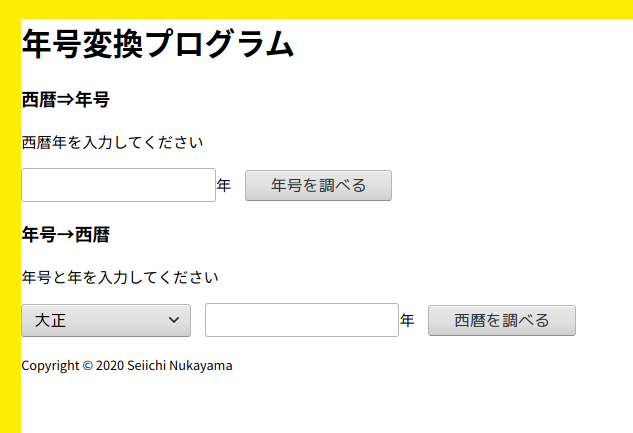
\includegraphics[width=10cm]{gamen01.png}

\subsubsection{処理の流れ}

おおまかに、どういう処理の流れにするかを考えます。

これは一つの例です。
ファイル名も例です。

\textgt{選択肢1}
\begin{enumerate}
 \item 入力画面で西暦を入力 (index.jsp)
 \item 西暦から年号と年を調べるサーブレットで受け取る (Xnengo.java)
 \item (サーブレットの中の処理) Nengo.class を使って、年号を求める (Nengo.java)
 \item 求めた年号と年を入力画面に返す。 (Xnengo.java)
 \item 入力画面で表示 (index.jsp)
\end{enumerate}

\textgt{選択肢2}
\begin{enumerate}
 \item 入力画面で年号と年を入力 (index.jsp)
 \item 年号と年から西暦を調べるサーブレットで受け取る (Xseireki.java)
 \item (サーブレットの中の処理) Nengo.class を使って、西暦を求める (Nengo.java)
 \item 求めた西暦を入力画面に返す。 (Xseireki.java)
 \item 入力画面で表示 (index.jsp)
\end{enumerate}

\subsubsection{データの受け渡しの方法}

最初の入力画面(index.jsp)からサーブレット(Xnengo.java, Xseireki.java)へのデータの受け渡しは、\textgt{POST} を使うことにします。( GET でもいんですが、とりあえず)

サーブレット内で、西暦から年号への変換、年号から西暦への変換は、今までに作成した Nengo.java をそのまま使うことにします。\textgt{toNengo}メソッド、\textgt{toSeireki}メソッドがそのまま使えます。

サーブレットから入力画面(index.jsp)へのデータの受け渡しには、セッション変数を使うことにします。

サーブレット内で以下のような式を記述するだけでセッション変数を使えます。

\verb!HttpSession session = request.getSession(true);!


このように 変数session を宣言して、次のように使います。

\verb!session.setAttribute("nengo", nengo);!

これは、"nengo"というセッション変数に nengo という値をセットしています。

そして、これを入力画面(index.jsp)で、以下のように取り出します。

\begin{lstlisting}[numbers=none]
<%
nengo = session.getAttribute("nengo");
%>
\end{lstlisting}

そして、これを \verb!<html><body>~</body><html>! の \verb!<body>!の中で、
\verb!<%= nengo %>! とすることで、画面に表示できます。




\end{document}

%% 修正時刻: Sat May  2 15:10:04 2020



%% 修正時刻: Tue May 12 06:42:11 2020
